% METODOLOGIA------------------------------------------------------------------

\chapter{Implementação do Protótipo}
\label{chap:prototipo}

Este capitulo descreve a montagem do protótipo para testes. Será feita uma introdução do funcionamento geral, e suas principais características. Posteriormente será mostrado o funcionamento da base de testes da câmera, conexões entre os servo motores e os pinos GPIO, instalação e configuração do sistema operacional para o Raspberry Pi, e desenvolvimento do programa e controle dos servo motores, desenvolvimento do aplicativo Android, responsável por capturar dados dos sensores de posição e envio pela rede sem fio.

\section{Especificação do Projeto}
\label{sec:especificacao}

Apesar de ser composto por diversos módulos, o projeto pode ser dividido conceitualmente em duas partes, denominados por módulo de coleta de dados, ou celular Android, e módulo de controle de câmera, ou Raspberry Pi. O módulo de controle de câmera é responsável por receber os dados de posição através de uma conexão socket, converter o sistema de coordenadas, aplicar um filtro para evitar o acionamento desnecessário dos motores e acionar os servos, quando necessário. O módulo de coleta de dados é responsável por configurar os sensores de localização disponíveis no smartfone, aplicar os filtros necessários para minimizar ruídos na coleta de dados, encontrar o módulo de controle de câmeras através de uma busca na rede e enviar para ele, os dados das coordenadas através de uma conexão socket. \par

\begin{figure}[H]
	\centering
	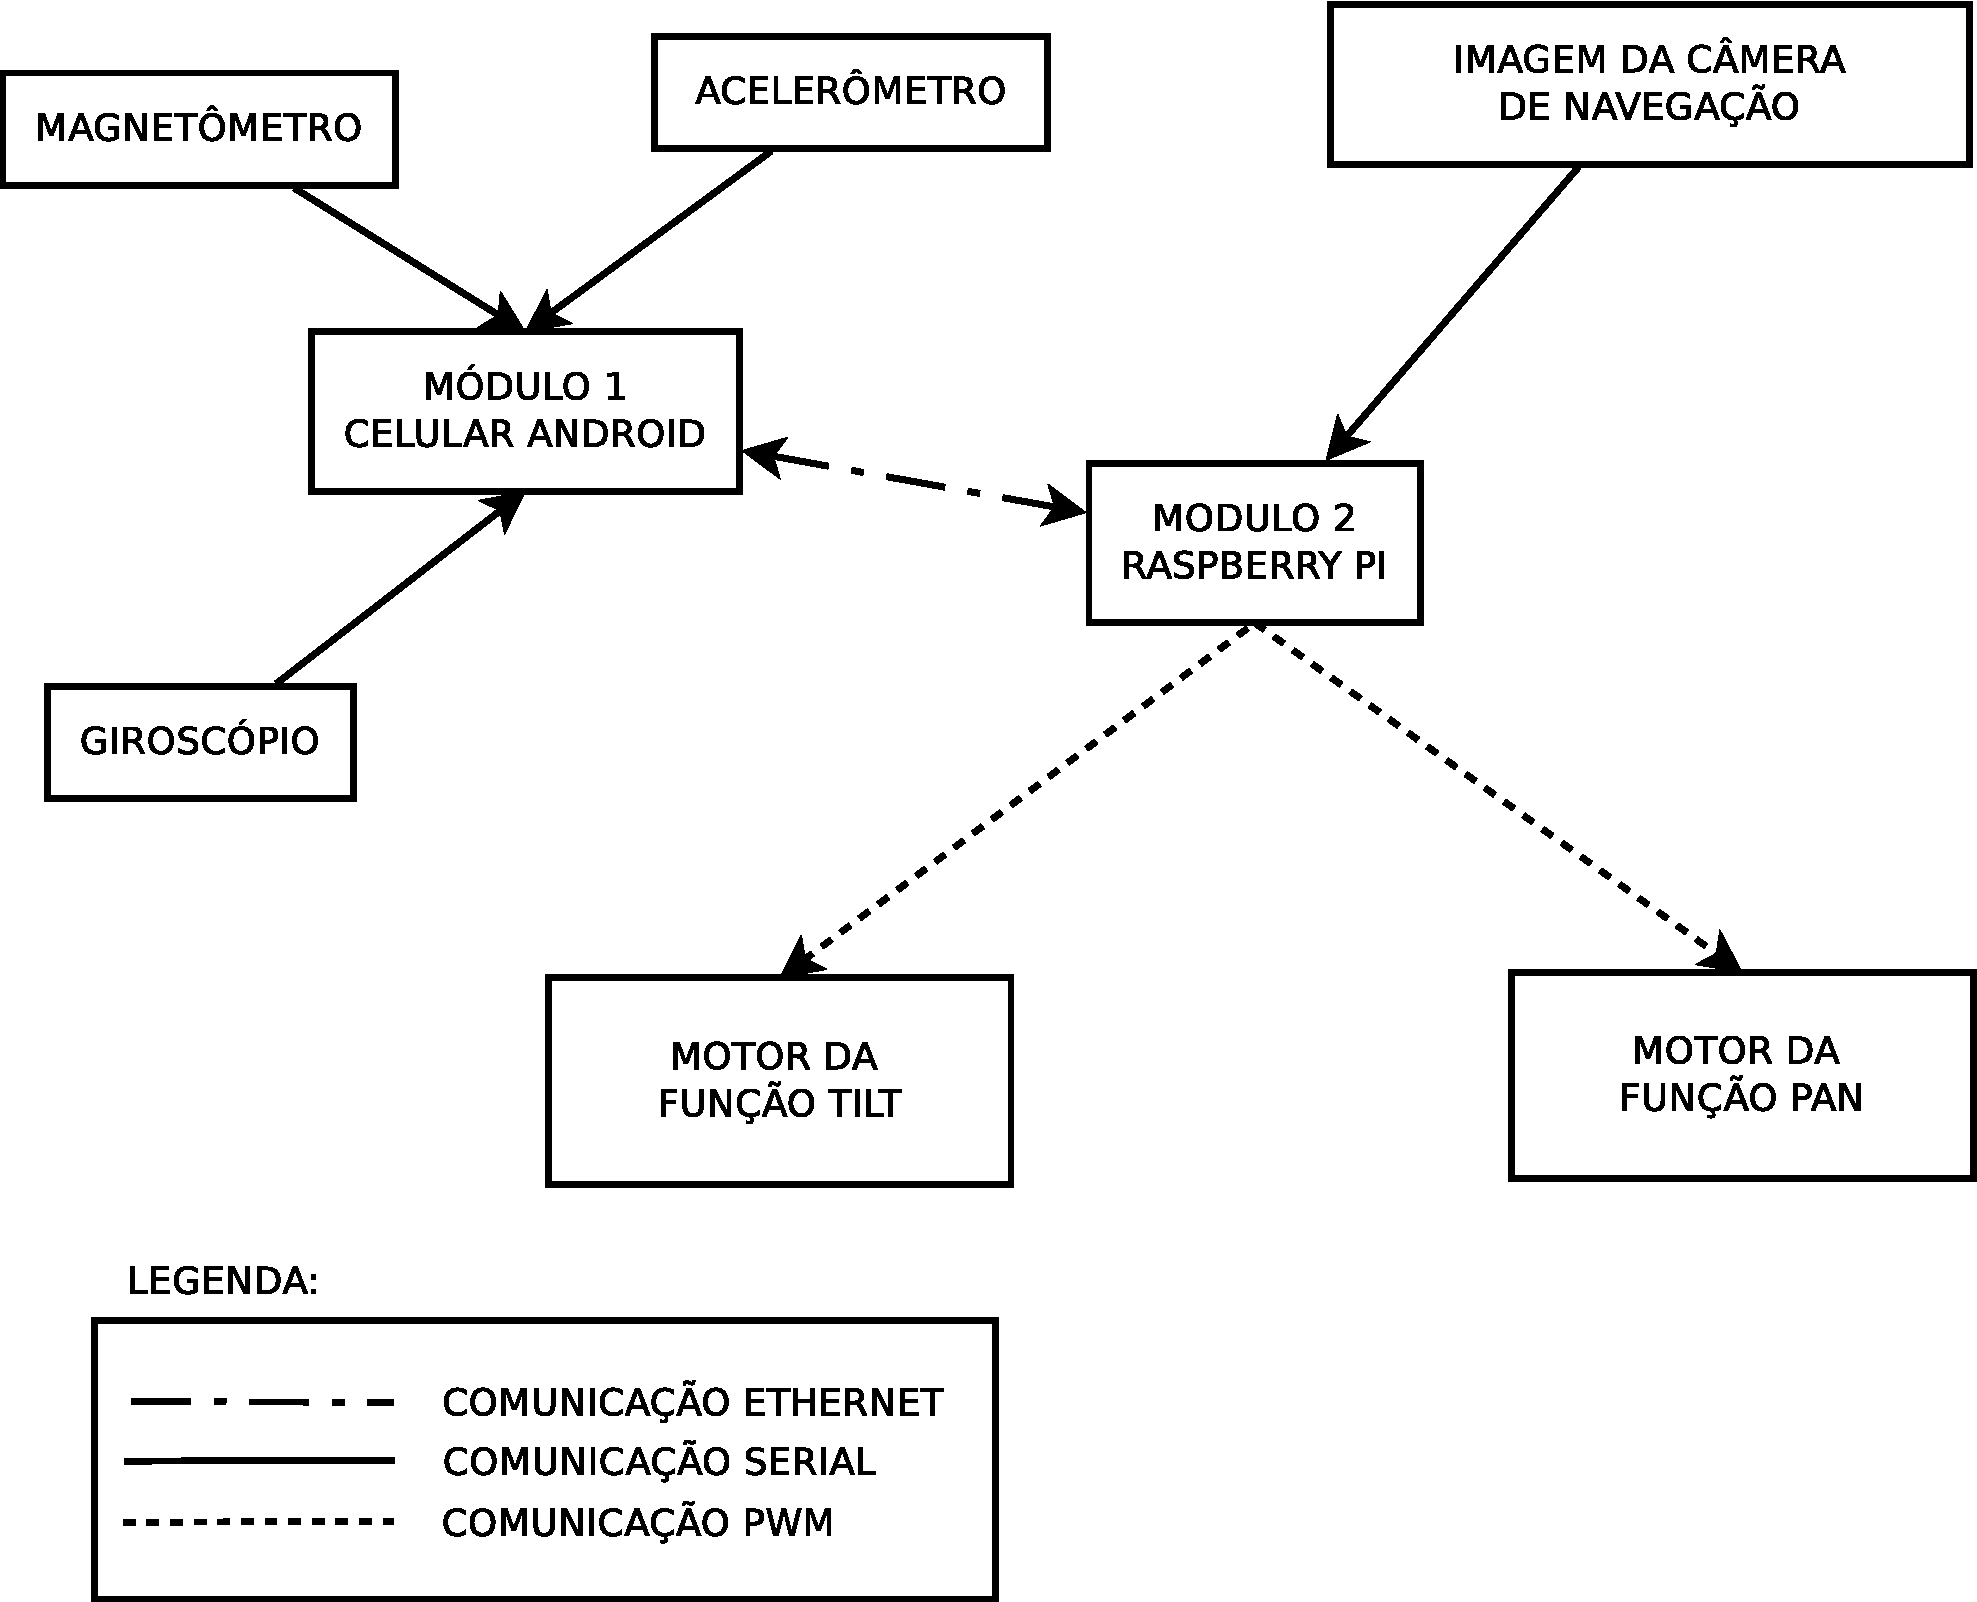
\includegraphics[width=0.7\textwidth]{figuras/diagrama-modulos-eps-converted-to.pdf}
	\caption{Diagrama de blocos da comunicação entre os módulos}
	\label{fig:diagrama_blocos}
\end{figure}

A \autoref{fig:diagrama_blocos} mostra como cada módulo se comunica com seus sensores, atuadores e entre sí. Os sensores estão embarcados no smartfone e não serão controlados separadamente. O sistema operacional Android fornece uma abstração para o hardware, e portanto não será necessário configurar os sensores manualmente. 

\subsection{Módulo de Controle de Câmeras}
\label{subsec:modconcam}

O módulo de controle de câmeras consiste em um SoC Raspberry Pi 1 modelo B, que possui um processador ARM de 700MHz, 512Mb de memória RAM, 26 pinos de proposito geral (GPIO), dua portas USB e uma porta Ethernet. Que tem as seguintes responsabilidades:

\begin{itemize}
	\item Responder requisições broadcast particular que identifica o módulo
	\item Receber dados de posição de sensores
	\item Filtrar os dados recebidos para evitar acionamento desnecessário dos motores
	\item Traduzir coordenadas dos sensores para coordenadas das câmeras
	\item Acionar dois motores servos de acordo coordenadas recebidas
\end{itemize}

\subsection{Módulo de Captura de Movimento}
\label{subsec:modcapmov}

O módulo de envio de coordenadas é um smartfone Android Motorola G6 com processador ARM Qualcomm Snapdragon 450 1,8 GHz Octa-Core, 3GB de memoria RAM, conectividade Wi-Fi, que possui os seguinte sensores: Acelerômetro, Magnetômetro, Giroscópio, Proximidade, Luz Ambiente e leitor de Impressão Digital. Que é responsável por:

\begin{itemize}
	\item Enviar requisição broadcast especial para detectar o módulo de controle de câmeras
	\item Conectar no módulo de controle de câmera
	\item Configurar sensores específicos para detecção de movimento
	\item Coletar dados dos sensores de movimento
	\item Aplicar filtro para evitar ruido na coleta dos dados de movimento
	\item Enviar coordenadas para o módulo de controle de câmera
\end{itemize}

\section{Montagem do Protótipo}
\label{sec:assemprototipo}

\subsection{Montagem do Módulo de Controle de Câmeras}
\label{subsec:assemmodconcam}

- instalação do SO\\
- configuração do SO\\
- instalação de pacotes necessarios para o desenvolvimento\\
- construção da classe server\\
- construção da classe servo\\
- construção da classe display\\
- construção da classe main\\

\subsection{Montagem do Módulo de Captura de Movimento}
\label{subsec:assemmodcapmov}

- instalação de pacotes necessarios para o desenvolvimento\\
- construção da classe Orientation\\
- construção da classe NetWorks\\
- construção da classe FullscreenActivity\\
